\section{Presentation of Results} \label{sec:res-presentation}

This section details the outcomes of experiments that aimed to develop and evaluate generative \ac{AI} models for audio production. The chief objectives of these experiments were to explore the potential of these models to generate audio with exceptional quality and to assess their performance in various circumstances. The experiments addressed specific research questions and hypotheses. 

This section presents a thorough summary of the experiments conducted in this research. Each experiment was intentionally designed to evaluate and test the effectiveness of the generated \ac{AI} models for audio.

Each experiment begins with an introduction that highlights the motivation and specific objectives, thereby establishing the context and rationale for the experiment. In addition, the text provides a detailed description of the hardware, software, and architecture used in each experiment to ensure transparency and reproducibility.

The performance of the generative \ac{AI} models is assessed by presenting line plots showing the evolving losses throughout the training process. In addition, spectrograms are displayed to visually represent the generated audio, allowing a qualitative evaluation of the model's performance.

By systematically organizing the experimental details, a thorough understanding of the experimental procedure and results is established. This section provides the basis for analyzing and discussing the effectiveness of the generative \ac{AI} models. These results can also be seen in table format in Appendix~\ref{ann:ganmix-results}.

\subsection{Experiment 1: Initial Model Evaluation} \label{sec:exp1}

The objective of Experiment 1 was to assess the initial model's performance and to establish a baseline for future development in generative model research. The goals were to appraise the model's ability to produce realistic audio and to analyze its training process.

The initial model comprised about 4 million parameters, evenly distributed between the generator and the discriminator. The model was trained using the \ac{BCE} loss function, and no regularization techniques were applied in this experiment.

The Audio MNIST dataset was used for both training and evaluation. The Adam optimizer with a learning rate of $1 \times 10^{-4}$ was used for the generator and discriminator. Throughout the training, the generator loss was calculated as $0.487$, while the discriminator loss was measured to be $1.440$. The total loss, which is the sum of the generator and discriminator losses, was calculated to be $1.927$.

Upon evaluation, it was determined that the initial model's spectrogram did not resemble actual audio. However, the training process quickly stabilized.

Figure \ref{fig:exp1_loss} presents a line plot of the continual losses during the training process for Experiment 1, providing insight into the model's learning progress and convergence. Additionally, the spectrogram generated by the initial model is depicted in Figure \ref{fig:exp1_spectrogram}, providing a visual assessment of the audio created.

\begin{figure}[!ht]
    \centering
    \begin{subfigure}{0.45\textwidth}
        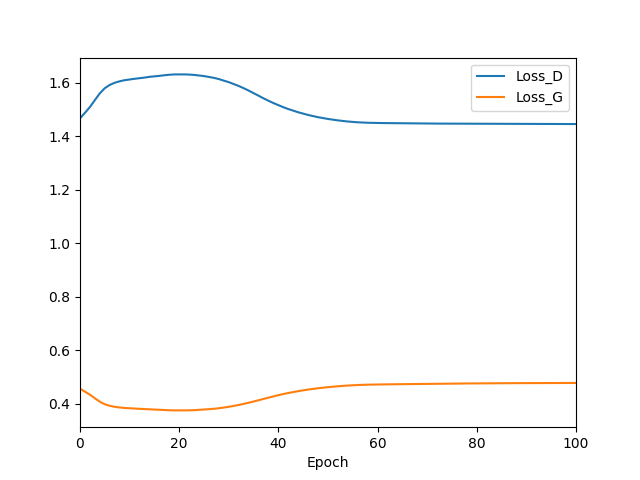
\includegraphics[width=\textwidth]{figures/4.5-results/exp1_loss.png}
        \caption{Evolving losses throughout the training process for Experiment 1.}
        \label{fig:exp1_loss}
    \end{subfigure}
    \begin{subfigure}{0.45\textwidth}
        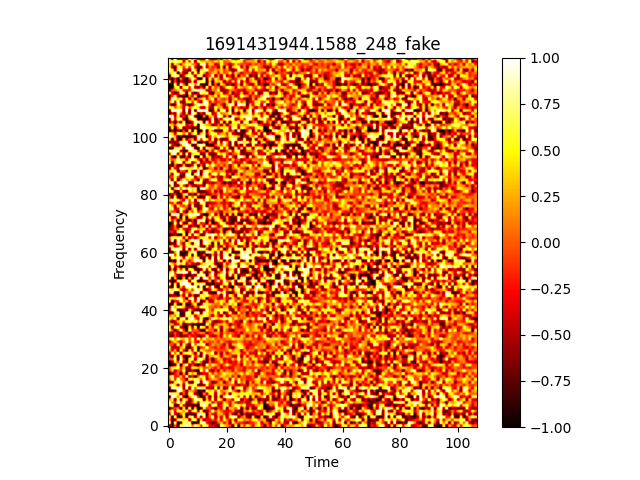
\includegraphics[width=\textwidth]{figures/4.5-results/exp1_spectrogram.png}
        \caption{Spectrogram generated in Experiment 1.}
        \label{fig:exp1_spectrogram}
    \end{subfigure}
    \caption{Results of Experiment 1.}
    \label{fig:exp1_results}
\end{figure}
\subsection{Experiment 2: Accelerating Convergence through Elevated Learning Rates} \label{sec:exp2}

Given the extended convergence observed during the initial experiment, the author deliberated on a strategic approach to hasten the convergence rate. This led to the contemplation of raising the learning rates as a feasible method of accelerating the convergence process.

This model shared the same number of parameters (about 4 million), loss function (\ac{BCE}), dataset, optimizer, and hardware setup as the former one.

The learning rate, for both the generator and the discriminator, was elevated to $1 \times 10^{-2}$. At the conclusion of the training process, the generator’s loss was calculated at $0.545$, and the discriminator’s loss was measured at $1.412$. The total loss, represented as the cumulative sum of the generator and discriminator losses, was calculated at $1.957$.

Upon evaluation, the spectrogram of the initial model was determined to be similar to the first one. The point at which the models began learning at a slower rate was reached more quickly, but the outcomes remained unsatisfactory.

Figure~\ref{fig:exp2_results} shows the loss and final spectrogram produced.

\begin{figure}[!ht]
    \centering
    \begin{subfigure}{0.45\textwidth}
        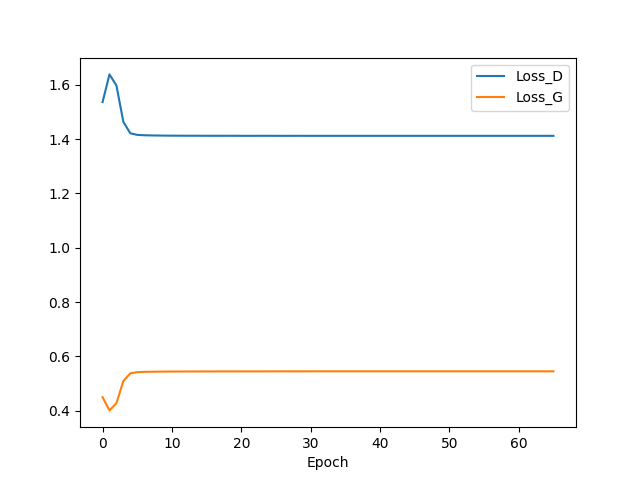
\includegraphics[width=\textwidth]{figures/4.5-results/exp2_loss.png}
        \caption{Evolving losses throughout the training process for Experiment 2.}
        \label{fig:exp2_loss}
    \end{subfigure}
    \begin{subfigure}{0.45\textwidth}
        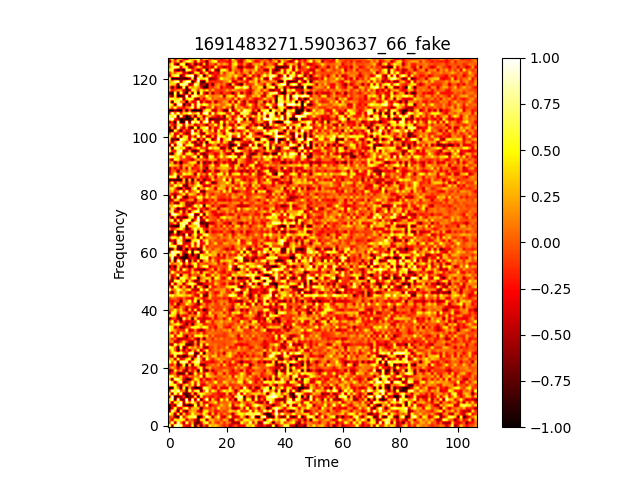
\includegraphics[width=\textwidth]{figures/4.5-results/exp2_spectrogram.png}
        \caption{Spectrogram generated in Experiment 2.}
        \label{fig:exp2_spectrogram}
    \end{subfigure}
    \caption{Results of Experiment 2.}
    \label{fig:exp2_results}
\end{figure}
\subsection{Experiment 3: Enhancing Performance through Learning Rate and Model Complexity}

Experiment 3 was designed to test two hypotheses aimed at improving the generative model's performance. The first hypothesis assumes that setting a higher learning rate for the generator than for the discriminator at the outset could enhance performance. The second hypothesis suggests that improving the generator model's complexity could lead to better results. These hypotheses stem from the assumption that the generator task is more challenging than the discriminator task.

For this experiment, the discriminator model remained unchanged while the generator model had significantly more trainable parameters, totaling about 25 million. This was done by increasing the number of filters and the number of convolutional layers per deconvolutional block. The experiment utilized the same loss function (\ac{BCE}), dataset, optimizer, and hardware configuration as the previous iterations.

To test the hypotheses, the author derived the learning rates from the initial experiment. The generator learning rate was increased to $1 \times 10^{-3}$, while the discriminator learning rate remained at $1 \times 10^{-4}$. Training for this model stopped after 14 epochs because the results were comparable to those of the first iteration.

The total loss was $2.037$, calculated by adding the generator loss of $0.351$ and the discriminator loss of $1.686$.

Figure~\ref{fig:exp3_results} presents the loss and final spectrogram generated in this experiment.

\begin{figure}[!ht]
    \centering
    \begin{subfigure}{0.45\textwidth}
        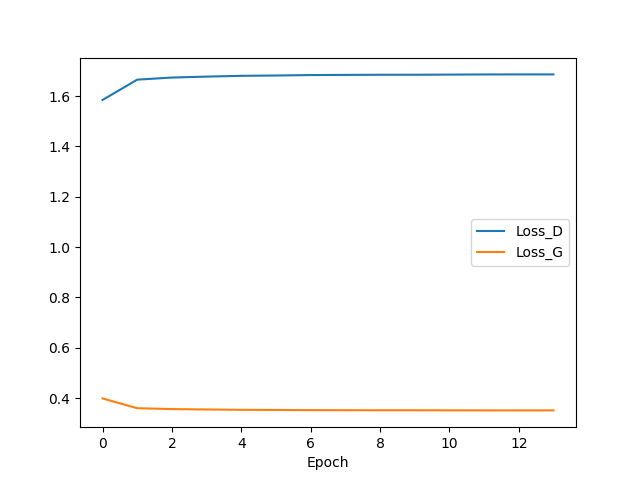
\includegraphics[width=\textwidth]{figures/4.5-results/exp3_loss.png}
        \caption{Evolving losses throughout the training process for Experiment 3.}
        \label{fig:exp3_loss}
    \end{subfigure}
    \begin{subfigure}{0.45\textwidth}
        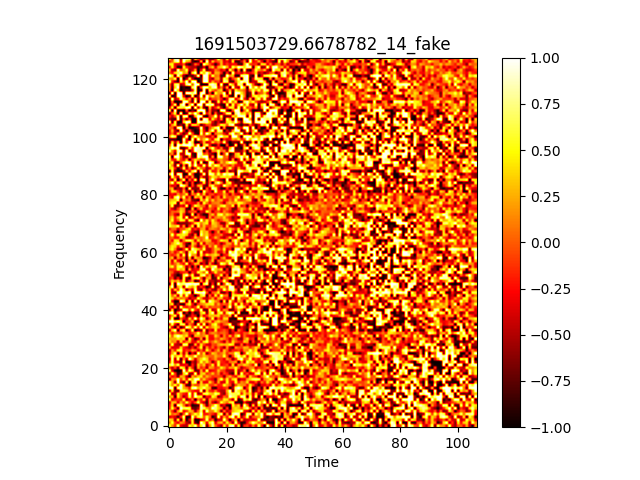
\includegraphics[width=\textwidth]{figures/4.5-results/exp3_spectrogram.png}
        \caption{Spectrogram generated in Experiment 3.}
        \label{fig:exp3_spectrogram}
    \end{subfigure}
    \caption{Results of Experiment 3.}
    \label{fig:exp3_results}
\end{figure}
\subsection{Experiment 4: Comparing Optimization Algorithms: RMSProp and SGD} \label{sec:exp4}

Experiment 4 tested two optimization algorithms on the generative models.

The experiment examined the performance of the RMSProp and \ac{SGD} optimizers, in contrast to the previous experiments that relied on the Adam optimizer.

This experiment utilized identical model architecture, loss function (\ac{BCE}), and dataset as Experiment 3. The code was transferred to \ac{LIACC} 1 hardware configuration, with minimal alterations.

The initial experiment in this set utilized the RMSProp optimizer's default settings. The comprehensive loss was $1.966$, comprising a generator loss of $0.558$ and a discriminator loss of $1.407$.

Figure~\ref{fig:exp4_rms_results} offers insight into the loss and last spectrogram produced during this trial.

The next experiment in the sequence employed the standard configuration of the \ac{SGD} optimizer (for specifics, see Section~\ref{sec:sgd}). The total loss was calculated to be $1.945$, with a generator loss of $0.516$ and a discriminator loss of $1.429$.

Figure~\ref{fig:exp4_sgd_results} presents the loss and the final spectrogram generated in this experiment.

The obtained results were comparable to those obtained with the Adam optimizer in previous iterations.

\begin{figure}[!ht]
    \centering
    \begin{subfigure}{0.45\textwidth}
        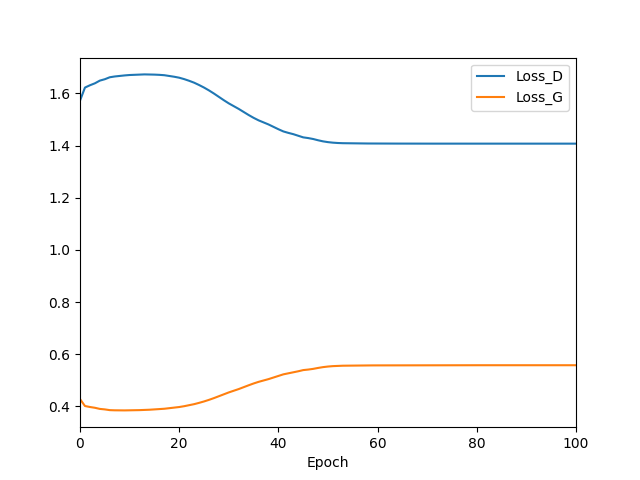
\includegraphics[width=\textwidth]{figures/4.5-results/exp4_rms_loss.png}
        \caption{Evolving losses throughout the training process for Experiment 4 with RMSprop.}
        \label{fig:exp4_rms_loss}
    \end{subfigure}
    \begin{subfigure}{0.45\textwidth}
        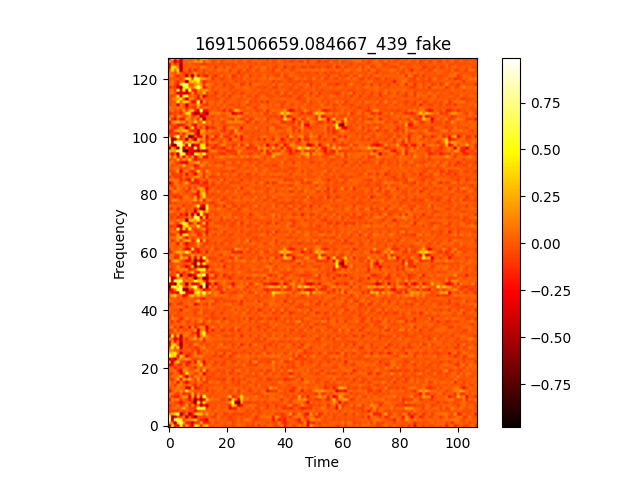
\includegraphics[width=\textwidth]{figures/4.5-results/exp4_rms_spectrogram.png}
        \caption{Spectrogram generated in Experiment 4 with RMSprop.}
        \label{fig:exp4_rms_spectrogram}
    \end{subfigure}
    \caption{Results of Experiment 4 with RMSprop.}
    \label{fig:exp4_rms_results}
\end{figure}

\begin{figure}[!ht]
    \centering
    \begin{subfigure}{0.45\textwidth}
        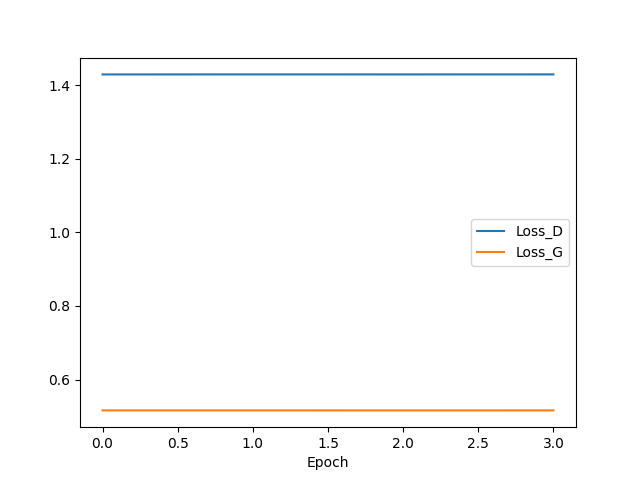
\includegraphics[width=\textwidth]{figures/4.5-results/exp4_sgd_loss.png}
        \caption{Evolving losses throughout the training process for Experiment 4 with \ac{SGD}.}
        \label{fig:exp4_sgd_loss}
    \end{subfigure}
    \begin{subfigure}{0.45\textwidth}
        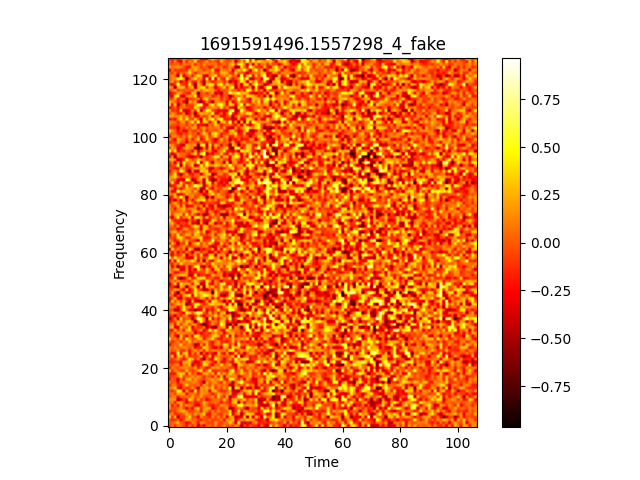
\includegraphics[width=\textwidth]{figures/4.5-results/exp4_sgd_spectrogram.png}
        \caption{Spectrogram generated in Experiment 4 with \ac{SGD}.}
        \label{fig:exp4_sgd_spectrogram}
    \end{subfigure}
    \caption{Results of Experiment 4 with \ac{SGD}.}
    \label{fig:exp4_sgd_results}
\end{figure}
\subsection{Experiment 5: Enhancing Performance with Regularization Techniques} \label{sec:exp5}

In this experiment, the author aimed to test the hypothesis that incorporating regularization techniques can enhance model performance. As such, several regularization techniques were utilized in the model. Initially, dropout layers were added, which randomly deactivate a percentage of neurons during training. This technique strengthens the model's ability to generalize. Batch normalization was included to normalize layer activations and decrease internal covariate shifts, speeding up training.

Additionally, the author introduced noise to the discriminator input to enhance model robustness, making it less sensitive to small perturbations and improving overall stability. Elastic network regularization, which combines both L1 and L2 penalties, was also utilized~\cite{zou_regularization_2005}.

It should be noted that the experimental setup was identical to Experiment 4, except for the use of the Adam optimizer. The total loss for this experiment was $4.791$, calculated by summing the generator loss of $3.362$ and the discriminator loss of $1.428$. However, it is important to note that comparing the current generator loss to previous results is not appropriate due to the incorporation of the elastic net regularization. This regularization method substantially elevates the generator loss but is crucial for training goals.

Regrettably, a flaw in the elastic net implementation was detected in the code, but not until after a few subsequent experiments. Although this error has a negative impact on the overall absolute loss and results, it does not affect the comparisons between experiments.

Refer to Figure~\ref{fig:exp5_results} for a visual representation of the results, displaying the loss and final spectrogram generated in this experiment.

\begin{figure}[!ht]
    \centering
    \begin{subfigure}{0.45\textwidth}
        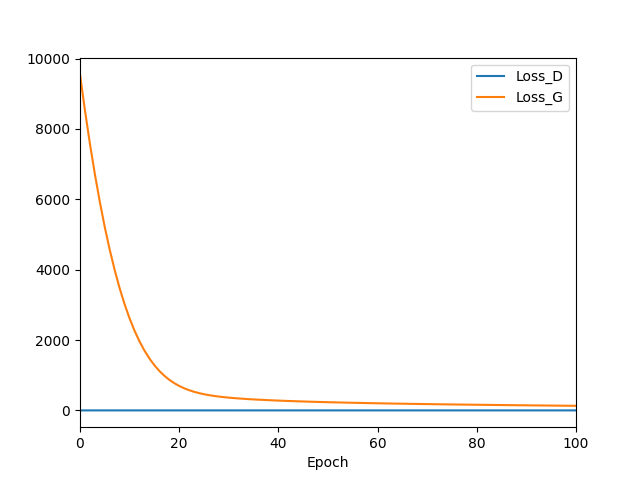
\includegraphics[width=\textwidth]{figures/4.5-results/exp5_loss.png}
        \caption{Evolving losses throughout the training process for Experiment 5.}
        \label{fig:exp5_loss}
    \end{subfigure}
    \begin{subfigure}{0.45\textwidth}
        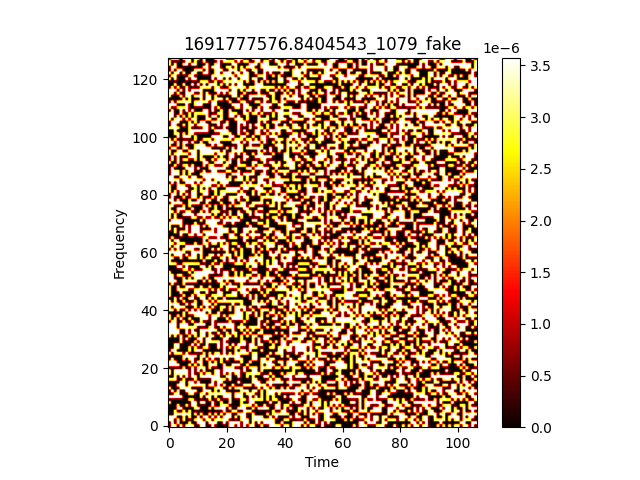
\includegraphics[width=\textwidth]{figures/4.5-results/exp5_spectrogram.png}
        \caption{Spectrogram generated in Experiment 5.}
        \label{fig:exp5_spectrogram}
    \end{subfigure}
    \caption{Results of Experiment 5.}
    \label{fig:exp5_results}
\end{figure}
\subsection{Experiment 6: Optimizing Model Balance} \label{sec:exp6}

In this experiment, the author aimed to leverage the upgraded hardware configuration of the \ac{LIACC} 2 system. After updating the model to include the Clotho dataset, which demanded more significant \ac{GPU} and \ac{RAM} resources, the results were analyzed.

Nevertheless, the author found them unsatisfactory, possibly due to the imbalance of the generator and discriminator models, with the former having about 25 million parameters and the latter having only about 2 million. Typically, \ac{GAN} models are designed as a pair of similar or mirrored models.

To mitigate this problem, the author reversed the model difference that was introduced in Experiment 3. The generator and discriminator models were both adjusted to have around 2 million parameters each.

The loss function, regularization techniques, and optimizer remained unchanged. The total loss for this experiment was $2.045$, calculated by adding the generator loss of $0.587$ and the discriminator loss of $1.458$.

For a visual representation of the results, which includes the loss and the final spectrogram generated in this experiment, please see Figure~\ref{fig:exp6_results}.

\begin{figure}[!ht]
    \centering
    \begin{subfigure}{0.45\textwidth}
        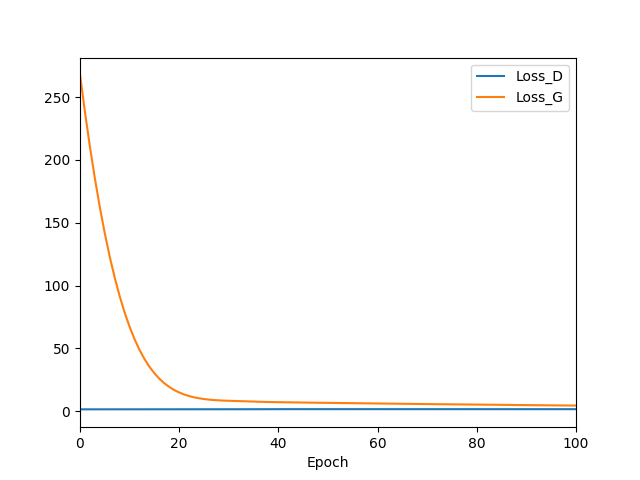
\includegraphics[width=\textwidth]{figures/4.5-results/exp6_loss.png}
        \caption{Evolving losses throughout the training process for Experiment 6.}
        \label{fig:exp6_loss}
    \end{subfigure}
    \begin{subfigure}{0.45\textwidth}
        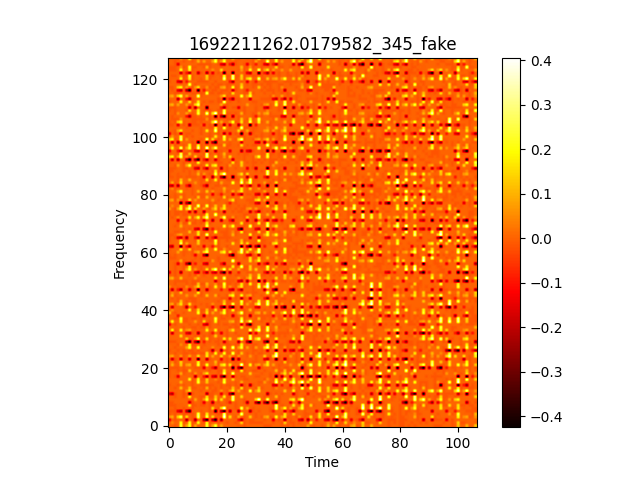
\includegraphics[width=\textwidth]{figures/4.5-results/exp6_spectrogram.png}
        \caption{Spectrogram generated in Experiment 6.}
        \label{fig:exp6_spectrogram}
    \end{subfigure}
    \caption{Results of Experiment 6.}
    \label{fig:exp6_results}
\end{figure}
\subsection{Experiment 7: Scaling Complexity} \label{sec:exp7}

Building upon the success of the previous experiment, the purpose of this study was to replicate the same approach utilizing larger models. This was achieved by amplifying the number of convolutional layers in each block and the number of filters in each convolutional layer.

This experiment tested two sets of models. The first set comprised of models, each with 10 million parameters, resulting in a total of 20 million parameters. The second set includes models with a total of 50 million parameters, each having 25 million parameters.

The other configuration aspects, such as the loss function, regularization techniques, data set, optimizer, and hardware configuration, remained the same.

In the initial test, the generator loss of $1.132$ and the discriminator loss of $1.389$ resulted in a total loss of $2.512$.

For a visual representation of the experiment results, including the loss and final spectrogram, please see Figure~\ref{fig:exp7_10_results}.

\begin{figure}[!ht]
    \centering
    \begin{subfigure}{0.45\textwidth}
        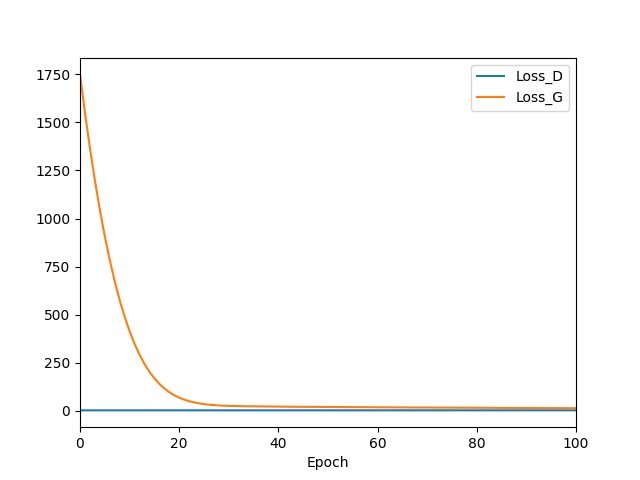
\includegraphics[width=\textwidth]{figures/4.5-results/exp7_10_loss.png}
        \caption{Evolving losses throughout the training process for Experiment 7 with 20 million parameters.}
        \label{fig:exp7_10_loss}
    \end{subfigure}
    \begin{subfigure}{0.45\textwidth}
        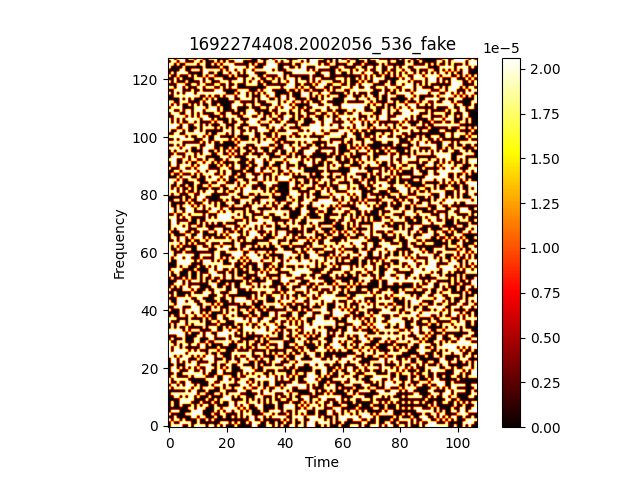
\includegraphics[width=\textwidth]{figures/4.5-results/exp7_10_spectrogram.png}
        \caption{Spectrogram generated in Experiment 7 with 20 million parameters.}
        \label{fig:exp7_10_spectrogram}
    \end{subfigure}
    \caption{Results of Experiment 7 with 20 million parameters.}
    \label{fig:exp7_10_results}
\end{figure}

The second experiment resulted in a total loss of $3.177$, comprising a generator loss of $1.738$ and a discriminator loss of $1.439$.

To view the experiment results, including the loss and final spectrogram, refer to Figure~\ref{fig:exp7_25_results}.

\begin{figure}[!ht]
    \centering
    \begin{subfigure}{0.45\textwidth}
        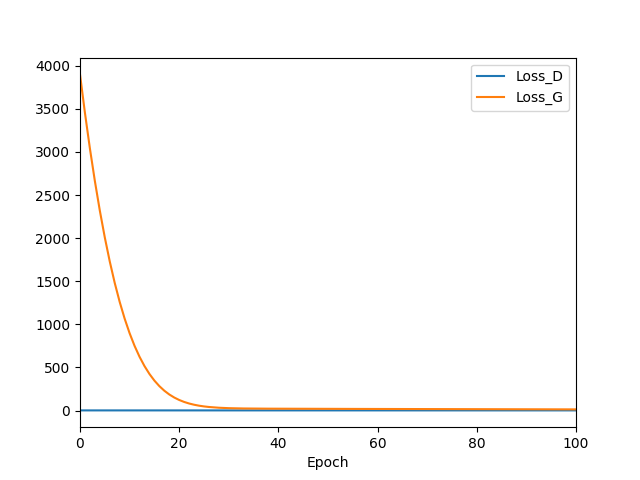
\includegraphics[width=\textwidth]{figures/4.5-results/exp7_25_loss.png}
        \caption{Evolving losses throughout the training process for Experiment 7 with 50 million parameters.}
        \label{fig:exp7_25_loss}
    \end{subfigure}
    \begin{subfigure}{0.45\textwidth}
        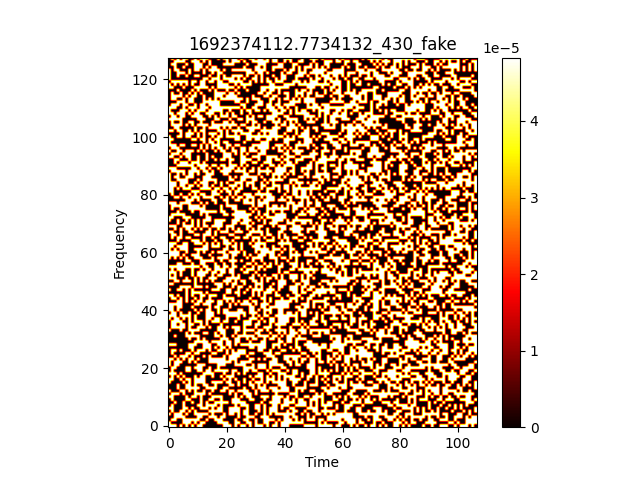
\includegraphics[width=\textwidth]{figures/4.5-results/exp7_25_spectrogram.png}
        \caption{Spectrogram generated in Experiment 7 with 50 million parameters.}
        \label{fig:exp7_25_spectrogram}
    \end{subfigure}
    \caption{Results of Experiment 7 with 50 million parameters.}
    \label{fig:exp7_25_results}
\end{figure}


\subsection{Experiment 8: Unregularized and Removal of Elastic Net} \label{sec:exp8}

In Experiment 5, a bug was identified and the author had to eliminate the elastic net implementation, which necessitated a complete rewrite of the models and training loop. Due to this, no regularization was enforced in this experiment.

However, aside from the absence of regularization and elastic net, the experimental setup is identical to the larger test performed in Experiment 7, which featured a model containing roughly 50 million parameters.

In epoch 37, the experiment incurred a total loss of $1.832$, consisting of the generator loss of $0.693$ and the discriminator loss of $1.139$.

Training of the model resulted in a sudden collapse at epoch 37, with inexplicable loss values plummeting to as low as 0 thereafter.

To gain insight into the training progress, two spectrograms were generated: one for epoch 37 (see Figure~\ref{fig:exp8_37_results}) and another for epoch 49, which marked the end of training (see Figure~\ref{fig:exp8_results}).

Additionally, a histogram depicting the values present in the generated encodings has been included in this experiment.

\begin{figure}[!ht]
    \centering
    \begin{subfigure}{0.4\textwidth}
        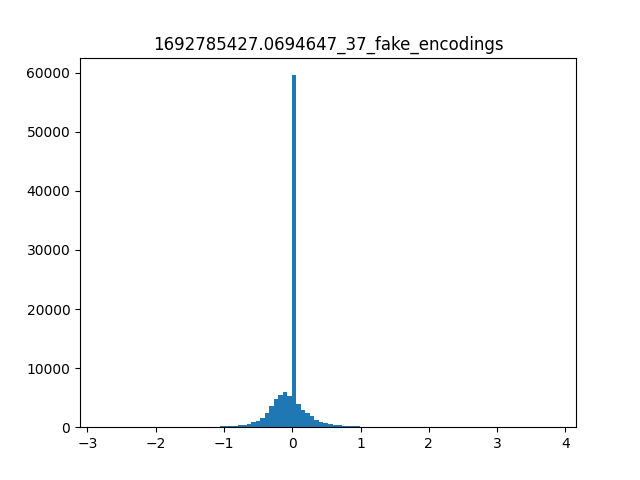
\includegraphics[width=\textwidth]{figures/4.5-results/exp8_37_hist.png}
        \caption{Histogram of the generated embeddings for Experiment 8 in epoch 37.}
        \label{fig:exp8_37_hist}
    \end{subfigure}
    \begin{subfigure}{0.4\textwidth}
        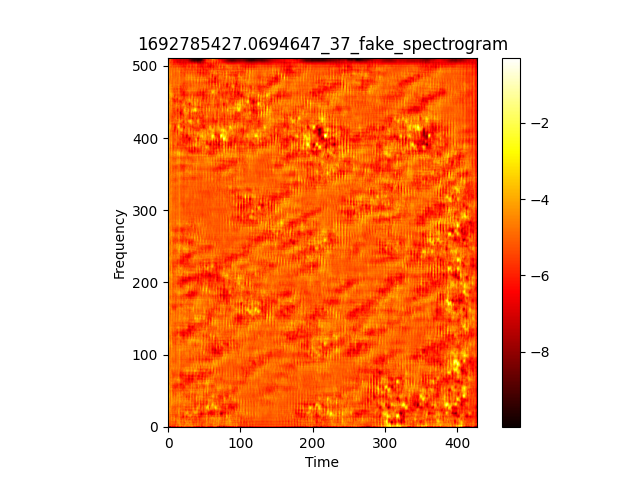
\includegraphics[width=\textwidth]{figures/4.5-results/exp8_37_spectrogram.png}
        \caption{Spectrogram generated in Experiment 8 in epoch 37.}
        \label{fig:exp8_37_spectrogram}
    \end{subfigure}
    \caption{Results of Experiment 8 in epoch 37.}
    \label{fig:exp8_37_results}
\end{figure}

\begin{figure}[!ht]
    \centering
    \begin{subfigure}{0.3\textwidth}
        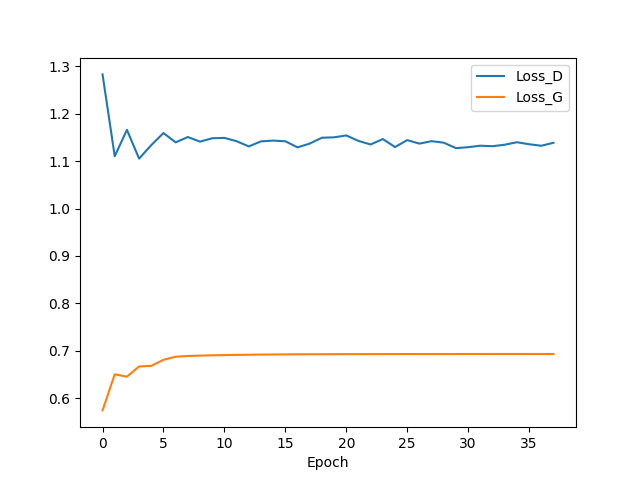
\includegraphics[width=\textwidth]{figures/4.5-results/exp8_loss.png}
        \caption{Evolving losses throughout the training process for Experiment 8.}
        \label{fig:exp8_loss}
    \end{subfigure}
    \begin{subfigure}{0.3\textwidth}
        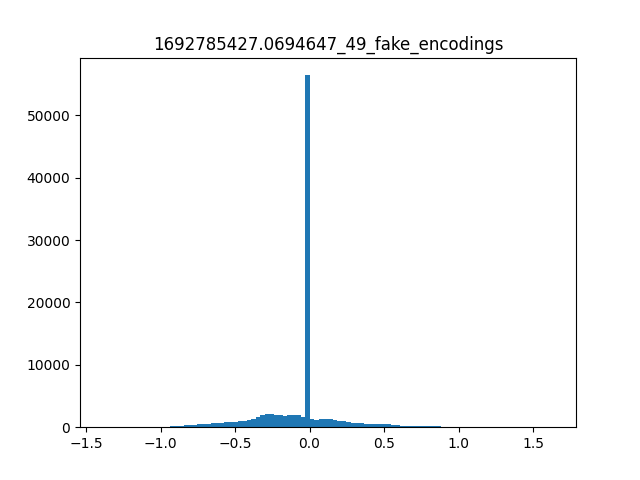
\includegraphics[width=\textwidth]{figures/4.5-results/exp8_hist.png}
        \caption{Histogram of the generated embeddings for Experiment 8.}
        \label{fig:exp8_hist}
    \end{subfigure}
    \begin{subfigure}{0.3\textwidth}
        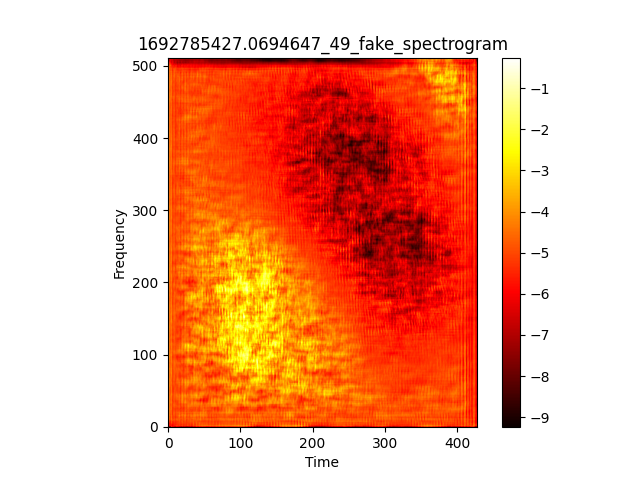
\includegraphics[width=\textwidth]{figures/4.5-results/exp8_spectrogram.png}
        \caption{Spectrogram generated in Experiment 8.}
        \label{fig:exp8_spectrogram}
    \end{subfigure}
    \caption{Results of Experiment 8 at the end of training.}
    \label{fig:exp8_results}
\end{figure}
\subsection{Experiment 9: Regularization Techniques and Training Progress for Rebuilt Model} \label{sec:exp9}

In this study, the author employed regularization techniques while holding all other parameters constant to build upon the previous experiment.

Nonetheless, an unforeseen crash transpired at epoch 34, resulting in a substantial reduction in loss values that ultimately converged to zero. It is crucial to note that all presented values are objective and exclusively quantitative.

The experiment incurred a total loss of $1.700$, with $0.693$ pertaining to the generator loss and $1.007$ to the discriminator loss.

To improve comprehension of the training progress, two spectrograms were produced: one for epoch 34 (refer to Figure~\ref{fig:exp9_34_results}) and the other for the final epoch, 49 (refer to Figure~\ref{fig:exp9_results}).

\begin{figure}[!ht]
    \centering
    \begin{subfigure}{0.4\textwidth}
        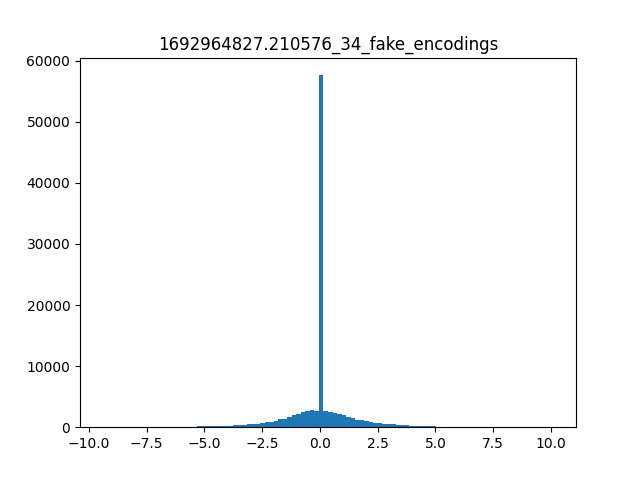
\includegraphics[width=\textwidth]{figures/4.5-results/exp9_34_hist.png}
        \caption{Histogram of the generated embeddings for Experiment 9 in epoch 34.}
        \label{fig:exp9_34_hist}
    \end{subfigure}
    \begin{subfigure}{0.4\textwidth}
        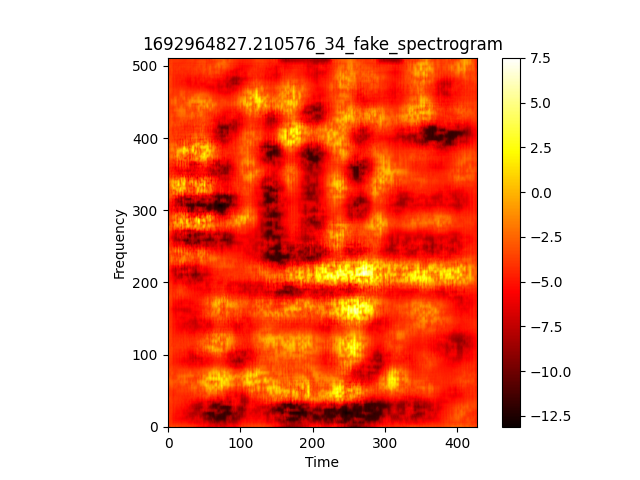
\includegraphics[width=\textwidth]{figures/4.5-results/exp9_34_spectrogram.png}
        \caption{Spectrogram generated in Experiment 9 in epoch 34.}
        \label{fig:exp9_34_spectrogram}
    \end{subfigure}
    \caption{Results of Experiment 9 in epoch 34.}
    \label{fig:exp9_34_results}
\end{figure}

\begin{figure}[!ht]
    \centering
    \begin{subfigure}{0.3\textwidth}
        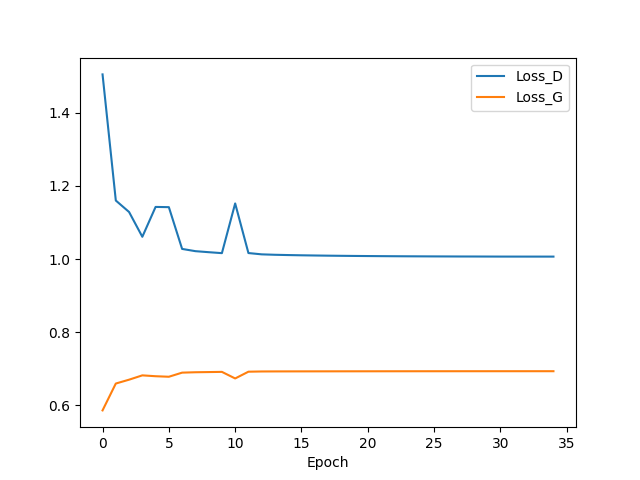
\includegraphics[width=\textwidth]{figures/4.5-results/exp9_loss.png}
        \caption{Evolving losses throughout the training process for Experiment 9.}
        \label{fig:exp9_loss}
    \end{subfigure}
    \begin{subfigure}{0.3\textwidth}
        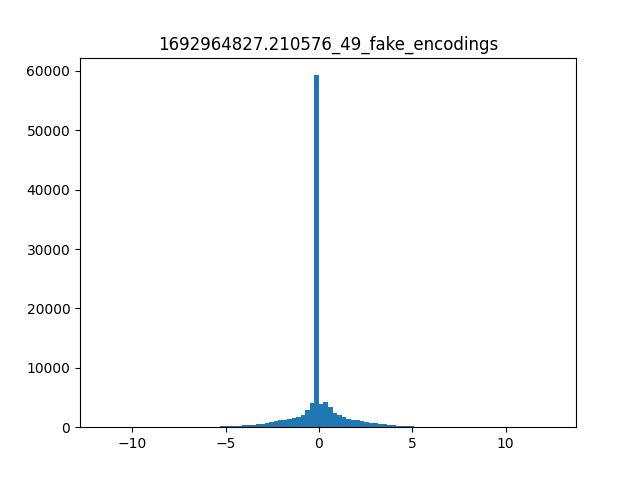
\includegraphics[width=\textwidth]{figures/4.5-results/exp9_hist.png}
        \caption{Histogram of the generated embeddings for Experiment 9.}
        \label{fig:exp9_hist}
    \end{subfigure}
    \begin{subfigure}{0.3\textwidth}
        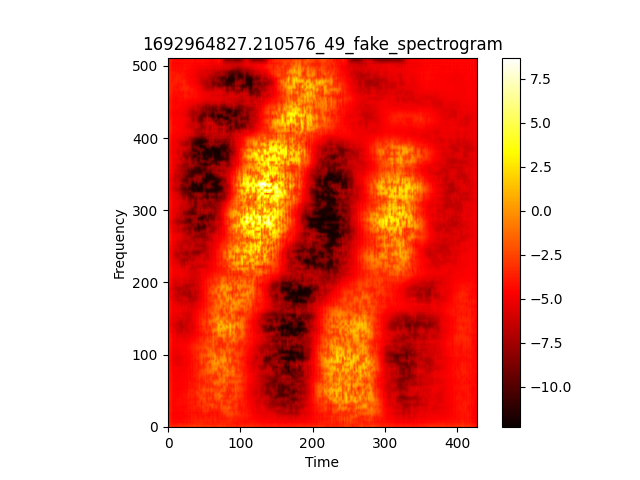
\includegraphics[width=\textwidth]{figures/4.5-results/exp9_spectrogram.png}
        \caption{Spectrogram generated in Experiment 9.}
        \label{fig:exp9_spectrogram}
    \end{subfigure}
    \caption{Results of Experiment 9 at the end of training.}
    \label{fig:exp9_results}
\end{figure}
\subsection{Experiment 10} \label{sec:exp10}

The GANmix model is made possible by the use of a pre-trained \ac{VAE}. In other words, the GANmix generator tries to generate encodings that are similar to those produced by the \ac{VAE}. The \ac{VAE} uses \acp{CNN}, which explains why the \ac{GAN} models also use encodings.

However, what the GANmix model actually produces are embeddings that have no significant spatial relationship.

This experiment builds on the notion that fully connected neural networks may provide better results.

To achieve this, the models were modified so that the generator has a connection (fully connected linear layer) from the input to the hidden layer, and another connection from the hidden layer to the output (the embeddings). The discriminator follows a similar model architecture.

Other configuration aspects such as loss function, regularization techniques, data set, optimizer, and hardware configuration remained unchanged.

The experiment incurred a total loss of $6.425$, with $6-987$ pertaining to the generator loss and $-0.562$ to the discriminator loss.

For a visual representation of the results, which includes the loss, the histogram of the generated embeddings and the final spectrogram generated in this experiment, please see Figure~\ref{fig:exp10_results}.

The data shows a curious pattern: the discriminator loss steadily decreases as the generator loss continuously increases. This trend could be due to insufficient epochs, problems with the optimizer, or the lack of a suitable scheduler. However, based on previous experiments, the criterion seems unlikely to be the primary cause.

\begin{figure}[!ht]
    \centering
    \begin{subfigure}{0.3\textwidth}
        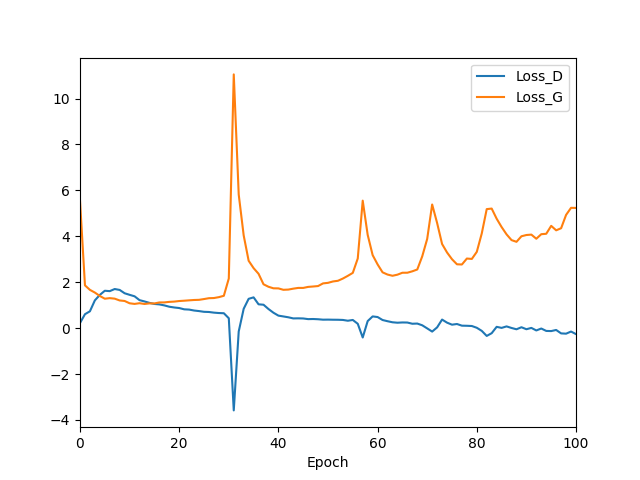
\includegraphics[width=\textwidth]{figures/4.5-results/exp10_loss.png}
        \caption{Evolving losses throughout the training process for Experiment 10.}
        \label{fig:exp10_loss}
    \end{subfigure}
    \begin{subfigure}{0.3\textwidth}
        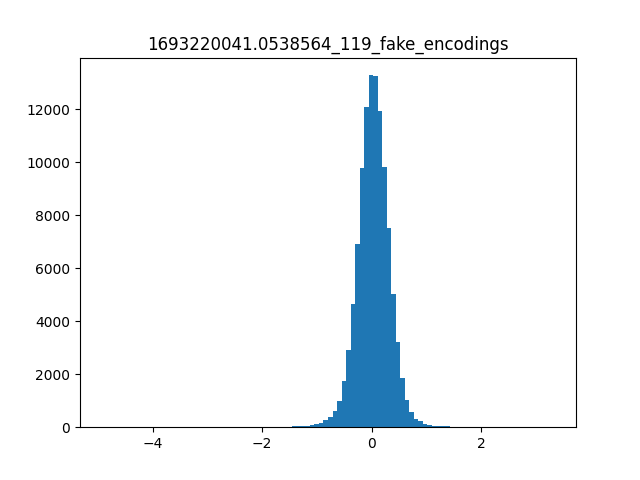
\includegraphics[width=\textwidth]{figures/4.5-results/exp10_hist.png}
        \caption{Histogram of the generated embeddings for Experiment 10.}
        \label{fig:exp10_hist}
    \end{subfigure}
    \begin{subfigure}{0.3\textwidth}
        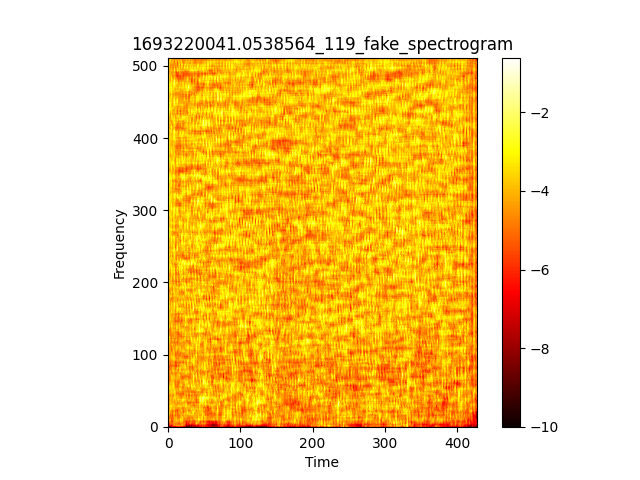
\includegraphics[width=\textwidth]{figures/4.5-results/exp10_spectrogram.png}
        \caption{Spectrogram generated in Experiment 10.}
        \label{fig:exp10_spectrogram}
    \end{subfigure}
    \caption{Results of Experiment 10.}
    \label{fig:exp10_results}
\end{figure}